% Editable LaTeX source. Build with Tectonic (XeTeX); see the companion .md.
\documentclass[a4paper,10pt]{article}
\usepackage[top=17mm,bottom=18mm,left=17mm,right=17mm]{geometry}
\usepackage{fontspec}
% Generated from comparison.json; rerun the PDF builder to refresh.
\newcommand{\DensityRows}{%
Exact particle sum & $0.47375505$ \\
Real-field/particle Gibbs, seed 1101 & $0.47113827 \pm 0.00095049$ \\
Real-field/particle Gibbs, seed 1201 & $0.47464444 \pm 0.00083619$ \\
Particle-only Gibbs, seed 2101 & $0.47479012 \pm 0.00115897$ \\
Historical native CL, seed 71 & $0.45115654 \pm 0.00333992$ \\
Historical native CL, seed 72 & $0.44947711 \pm 0.00337511$ \\
}

% Generated from comparison.json; rerun the PDF builder to refresh.
\newcommand{\HeightRows}{%
$4$ & $0.360268 \pm 0.000306$ & $0.360473 \pm 0.000374$ & $0.360899 \pm 0.000341$ \\
$16$ & $0.332038 \pm 0.000318$ & $0.331891 \pm 0.000292$ & $0.332504 \pm 0.000319$ \\
$32$ & $0.327538 \pm 0.000321$ & $0.328409 \pm 0.000294$ & $0.328293 \pm 0.000331$ \\
}

% Generated from comparison.json; rerun the PDF builder to refresh.
\newcommand{\PrlRows}{%
Neutral & $0.5065$ & $0.5066$ \\
$z_+=1$, mean field & $0.3144$ & $0.3210$ \\
$z_+=2$, mean field & $0.3562$ & $0.3491$ \\
$z_+=3$, mean field & $0.3824$ & $0.3705$ \\
$z_+=1$, LDA correlations & $0.3392$ & $0.3692$ \\
$z_+=2$, LDA correlations & $0.5817$ & $0.5562$ \\
$z_+=3$, LDA correlations & $0.7379$ & $0.7231$ \\
}

% Generated from comparison.json; rerun the PDF builder to refresh.
\newcommand{\ClosureRows}{%
$1$ & $0.0300$ & $0.0212$ & $0.0315$ \\
$2$ & $0.0298$ & $0.0088$ & $0.0301$ \\
$3$ & $0.0192$ & $0.0228$ & $0.0081$ \\
}

\usepackage{amsmath,amssymb,bm}
\usepackage{graphicx,booktabs,tabularx,array}
\usepackage[table]{xcolor}
\usepackage{pdflscape,fancyhdr}
\usepackage{pdfpages,eso-pic}
\usepackage[unicode,colorlinks=true,urlcolor=blue!55!black,linkcolor=blue!55!black]{hyperref}
\graphicspath{{prl_comparison_figs/oned_prl_20260907/}}
\definecolor{heading}{HTML}{12304A}
\definecolor{muted}{HTML}{52606D}
\definecolor{panel}{HTML}{EAF2F6}
\setlength{\parindent}{0pt}
\setlength{\parskip}{6pt}
\setlength{\emergencystretch}{1em}
\renewcommand{\arraystretch}{1.24}
\linespread{1.1}
\pagestyle{fancy}
\fancyhf{}
\fancyfoot[L]{\scriptsize\color{muted}Validation update \enspace|\enspace 2026-09-07}
\fancyfoot[R]{\scriptsize\thepage}
\renewcommand{\headrulewidth}{0pt}
\renewcommand{\footrulewidth}{0.3pt}
\newcommand{\pagetitle}[2]{\pdfbookmark[0]{#1}{#2}%
  {\sffamily\bfseries\color{heading}\fontsize{21}{27}\selectfont #1\par}\vspace{5pt}}
\newcommand{\subhead}[1]{\par\vspace{5pt}{\sffamily\bfseries\large\color{heading}#1\par}\vspace{2pt}}
\newcommand{\smallnote}[1]{{\small\color{muted}#1\par}}
\newcommand{\gridmean}[1]{\overline{#1}}
\newcommand{\units}[1]{\,\mathrm{#1}}
\hypersetup{pdftitle={1D sampling and PRL SCFT validation},
  pdfauthor={langevin-fts research notes},pdfsubject={Validation update, 2026-09-07}}

\begin{document}
% New direct MC / LDA / MF comparison; numbers come from matched bulk runs.
% Generated from concentration-matched comparison.json
\newcommand{\MCScftZeroMC}{$58.561$}
\newcommand{\MCScftZeroLDA}{$50.911$}
\newcommand{\MCScftZeroMF}{$59.602$}
\newcommand{\MCScftBathShift}{$0.053$}
\newcommand{\MCScftMaxMfHeightDifference}{$2.607$}
\newcommand{\MCScftHeightRows}{%
$1$ & $54.63\pm0.26$ & $46.34$ & $54.83$ \\
$2$ & $46.02\pm0.21$ & $29.38$ & $46.94$ \\
$3$ & $39.28\pm0.35$ & $14.12$ & $40.37$ \\
}
\newcommand{\MCScftChargeRows}{%
$\overline\Gamma_{0.5}$ & $0.310\pm0.004$ & $-0.397$ & $0.324$ \\
$\Psi_{\rm rel}$ & $-0.599\pm0.244$ & $0.784$ & $-0.860$ \\
}

\pagetitle{Sampling versus PRL-type SCFT}{mcscftheight}
\smallnote{Matched physical parameters and measured bulk concentrations\quad /\quad 2026-09-07}
\textbf{Result: the 1D samples are closer to mean-field SCFT with correlations disabled.}
Blue denotes actual MC samples; red denotes the existing PRL-type smoothed-LDA SCFT;
green denotes SCFT with correlation self-energies disabled, retaining the mean potential and canonical C.
Black squares are digitized paper theory curves, distinct from our LDA implementation.

\begin{center}
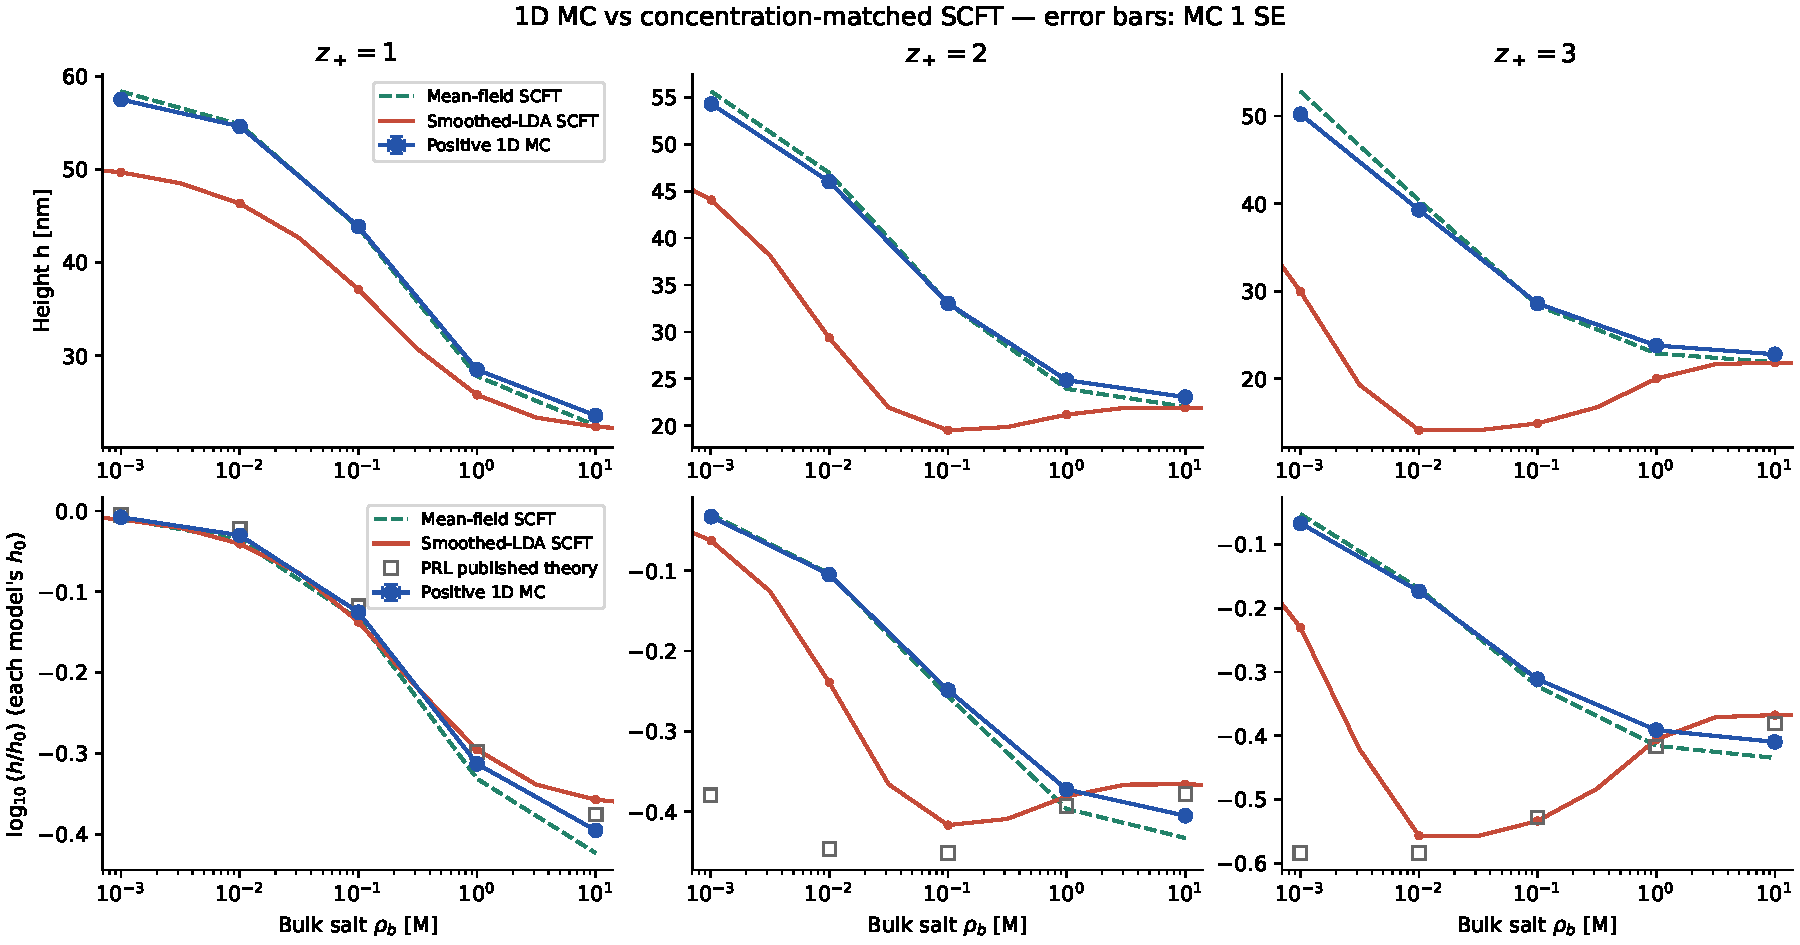
\includegraphics[width=\linewidth]{prl_comparison_figs/sampling_scft_20260907/mc_scft_height.pdf}
\end{center}
\vspace{-6pt}
\smallnote{Top: absolute height $h=2\int z\rho_P\,dz/(\sigma N)$.
Bottom: $\log_{10}(h/h_0)$, using each model's independently computed salt-free height.
MC error bars are 1 SE; the shared $h_0$ uncertainty correlates the normalized points.
Red lines show the earlier 19-point scan; small red dots are new solutions at the MC concentrations.}

\subhead{Heights near 0.01 M [nm]}
SCFT uses the actual MC bath concentration for each valence.

\begin{tabularx}{\linewidth}{@{}Xrrr@{}}
\toprule
\rowcolor{panel}$z_+$ & MC $\pm$ SE & LDA SCFT & Mean-field SCFT \\
\midrule
\MCScftHeightRows
\bottomrule
\end{tabularx}

Salt-free heights are MC \MCScftZeroMC\,nm, LDA \MCScftZeroLDA\,nm,
and mean field \MCScftZeroMF\,nm. These reference heights were not fitted to one another.
MC and mean field do not coincide: the largest absolute MC--MF height difference across
all comparison points is \MCScftMaxMfHeightDifference\,nm; some differences exceed the MC statistical errors.

\smallnote{$N=100$, $b=1\units{nm}$, $v=1\units{nm^3}$, $\sigma=0.1\units{nm^{-2}}$,
$\chi=0.5$, $\ell_B=0.7\units{nm}$, $a=0.25\units{nm}$, and $L=200\units{nm}$ were retained.
Replacing the nominal concentration with the measured MC bath concentration changes LDA heights by at most
\MCScftBathShift\,nm, insufficient to explain the large observed differences.
The paper uses a Gibbs dividing surface, so the normalized plot also compares different height definitions.}

\clearpage
\pagetitle{Charge, potential, and model differences}{mcscftcharge}
\begin{center}
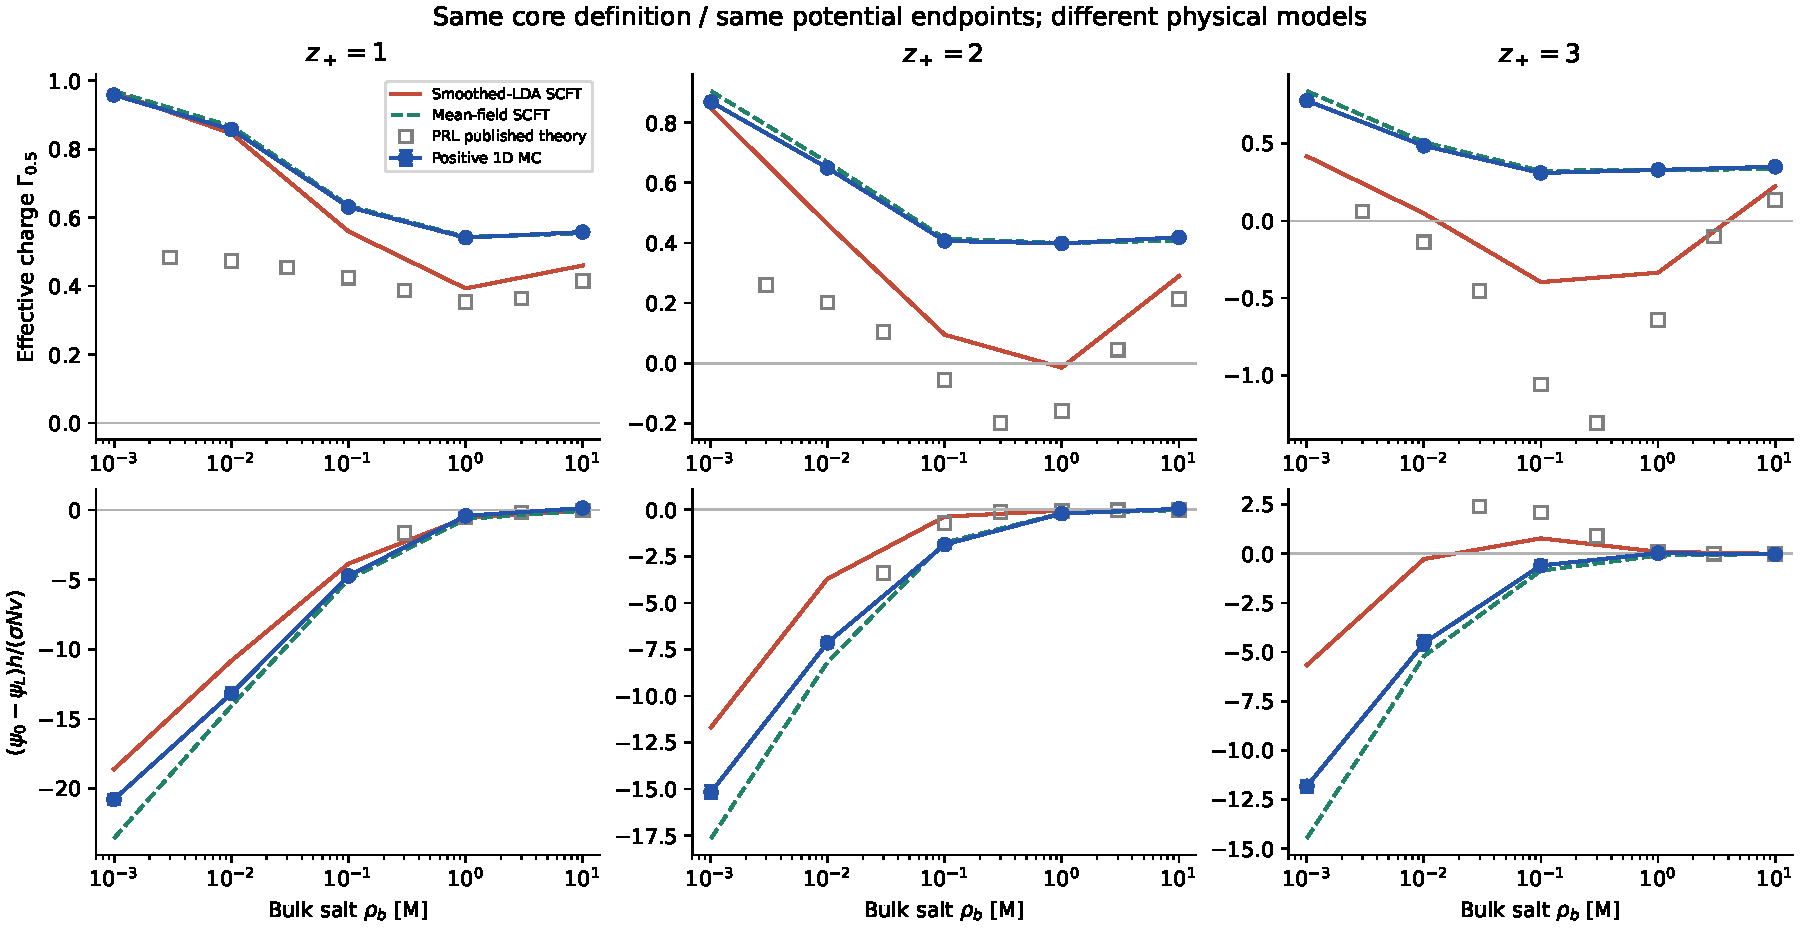
\includegraphics[width=\linewidth]{prl_comparison_figs/sampling_scft_20260907/mc_scft_charge.pdf}
\end{center}
\vspace{-7pt}
\smallnote{$\overline\Gamma_{0.5}$ is the salt-excess ratio in the core above half the polymer peak density.
SCFT densities were averaged over four cells onto the MC grid; potentials were compared at $z=0.25$, $199.75\units{nm}$.
This avoids mistaking an absolute gauge difference for potential reversal. Colors and symbols are as above.}

\subhead{Trivalent salt near 0.1 M: different charge and potential signs}
\begin{tabularx}{\linewidth}{@{}Xrrr@{}}
\toprule
\rowcolor{panel}Observable & MC $\pm$ SE & LDA SCFT & Mean-field SCFT \\
\midrule
\MCScftChargeRows
\bottomrule
\end{tabularx}

\subhead{A 1D mean profile can retain 3D fluctuations}
The PRL correlation theory includes a 3D charge Green function $G(\mathbf r,\mathbf r')$.
It retains transverse modes even for a planar mean density $\rho(z)$.
Its planar Fourier representation is
\begin{equation*}
 G(\mathbf r,\mathbf r')=
 \int\frac{d^2q_\parallel}{(2\pi)^2}
 e^{i\mathbf q_\parallel\cdot(\mathbf r_\parallel-\mathbf r'_\parallel)}
 G_{q_\parallel}(z,z')
\end{equation*}
The current MC samples a planar Coulomb action with only $q_\parallel=0$, excluding transverse fluctuations.
Increasing the sample count cannot restore those excluded correlation modes.
Our LDA approximates local 3D ionic correlations; equivalence to the paper's full nonlocal theory remains unverified.

This is a \textbf{comparison of different models}, not a test of MC algorithms for one action.
MC and MF also differ in finite $A$, integer cell solvent entropy, grid, charge smearing, and 1D fluctuations.
The PRL neglects $u_P^{\rm ex}$ but retains $u_P^0$; that omission alone cannot explain the discrepancy.
\smallnote{Theory: \href{https://arxiv.org/html/2404.09103v3}{Duan et al., Eqs.~(3)--(5)} and
SI Sec.~II. All new SCFT states passed full residual $10^{-7}$ and independent chain density/contour $Q$ checks at $10^{-10}$.
Numbers, density profiles, and run paths: \texttt{SAMPLING\_SCFT\_COMPARISON.md}.
The SCFT runs used the existing research runner; production FFT/C++/CUDA and MC/CL code were unchanged.}

\clearpage
% Actual stochastic sampling; separate from the older SCFT continuation.
% Generated from positive sampling analysis.json
\newcommand{\SamplingZeroHeight}{$58.56\pm0.35$}
\newcommand{\SamplingTinySigma}{2.67}
\newcommand{\SamplingRhatMax}{1.039}
\newcommand{\SamplingEssMin}{10.1}
\newcommand{\SamplingEssMax}{79.4}
\newcommand{\SamplingPairSigmaMax}{2.42}
\newcommand{\SamplingMaxChargeError}{$2.98e-12$}
\newcommand{\SamplingBathRelativeSe}{0.941}
\newcommand{\SamplingHeightRows}{%
$0.001$ & $57.52\pm0.36$ & $54.31\pm0.22$ & $50.21\pm0.29$ \\
$0.01$ & $54.63\pm0.26$ & $46.02\pm0.21$ & $39.28\pm0.35$ \\
$0.1$ & $43.88\pm0.17$ & $33.04\pm0.19$ & $28.60\pm0.33$ \\
$1$ & $28.49\pm0.21$ & $24.86\pm0.17$ & $23.80\pm0.19$ \\
$10$ & $23.57\pm0.14$ & $23.05\pm0.17$ & $22.80\pm0.29$ \\
}
\newcommand{\SamplingCheckRows}{%
Standard & $400$ & $40$ & $39.28\pm0.35$ \\
Finer grid & $800$ & $40$ & $39.18\pm0.20$ \\
Smaller area & $400$ & $20$ & $37.85\pm0.49$ \\
Larger area & $400$ & $80$ & $39.63\pm0.19$ \\
Salt-free, finer grid & $800$ & $40$ & $58.79\pm0.50$ \\
}
\newcommand{\SamplingControlSigma}{1.63}

\pagetitle{N=100 brush: Monte Carlo sampling}{positivesampling}
\smallnote{2026-09-07\quad /\quad New stochastic calculations, separate from the earlier Fig.~2--3 SCFT scan}

Sample averages were obtained by stochastic updates of incompressible P/S and ion configurations
and the real field in the attractive channel. Parameters were $N=100$, $b=1\units{nm}$,
$\sigma=0.1\units{nm^{-2}}$, $v=1\units{nm^3}$, $\chi=0.5$,
$\ell_B=0.7\units{nm}$, and $a=0.25\units{nm}$.

\textbf{Scope:} a finite planar model retaining only $z$, with 4 chains in $A=40\units{nm^2}$,
$L=200\units{nm}$, and $M=400$ cells. Transverse charge fluctuations are excluded,
so this differs from the paper's 3D statistical model. No LDA self-energy or PB/SCFT solution was inserted into the samples.

\begin{center}
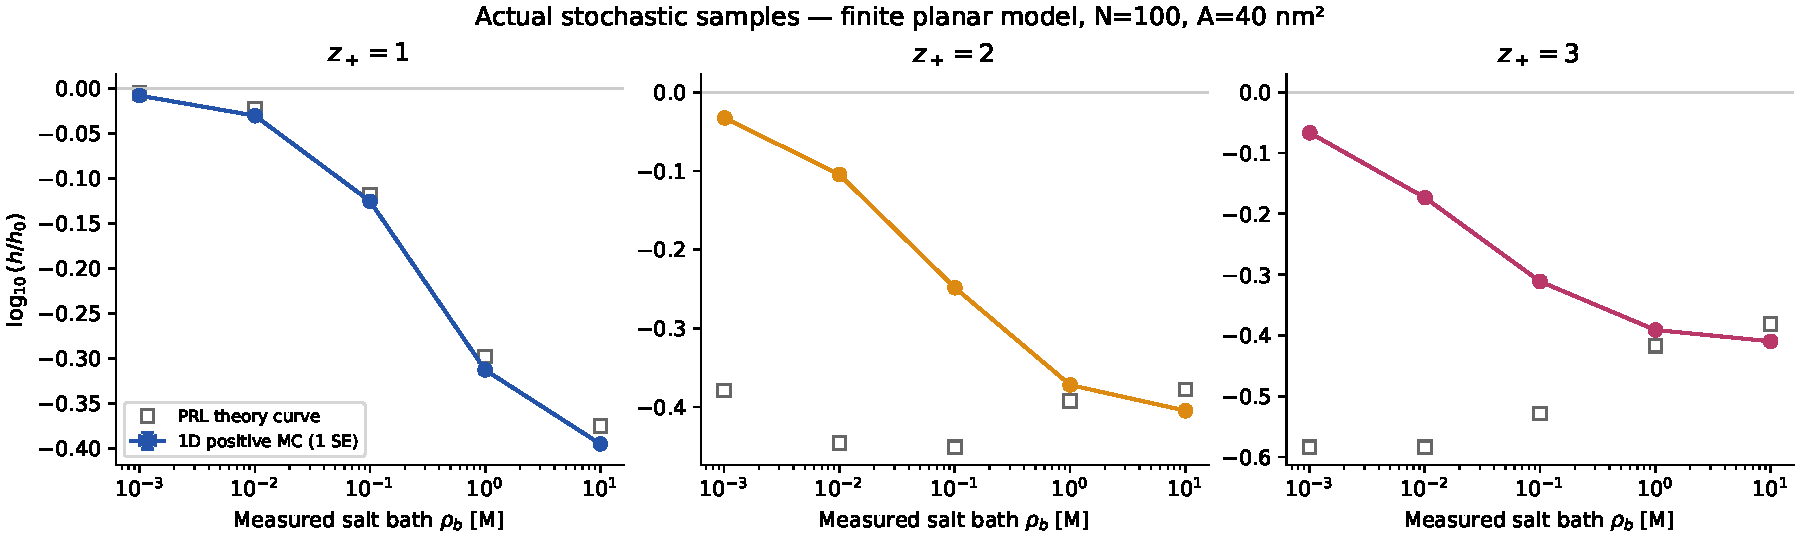
\includegraphics[width=\linewidth]{prl_comparison_figs/positive_brush_20260907/sampling_fig2.pdf}
\end{center}
\vspace{-6pt}
\smallnote{Circles and error bars: sample means and 1 SE. Open squares: digitized PRL theory curves.
The horizontal axis uses concentrations measured in separate pure-salt bulk simulations. The table lists nominal targets.}

\begin{tabularx}{\linewidth}{@{}Xrrr@{}}
\toprule
\rowcolor{panel}Target $\rho_b$ [M] & $z_+=1$: $h$ [nm] & $z_+=2$: $h$ [nm] & $z_+=3$: $h$ [nm] \\
\midrule
\SamplingHeightRows
\bottomrule
\end{tabularx}

\begin{equation*}
 h=\frac{2\int z\langle\rho_P(z)\rangle\,dz}{\sigma N}.
\end{equation*}
\smallnote{The salt-free reference was also sampled directly: $h_0=$\SamplingZeroHeight\,nm.
Height is explicitly defined by the first moment;
it is not automatically equivalent to the paper's Gibbs dividing-surface procedure.
Height decreases at the sampled concentrations, without reproducing the paper's pronounced re-expansion.}

\clearpage
\pagetitle{Sampled distribution and validation}{positivemeasure}
The cell capacity is $K=A\Delta z/v=20$. Polymer paths retain labeled bead coordinates;
solvent is eliminated exactly through $s_j=K-p_j$. Monovalent counterions are fixed at
$\sum_j c_j=n_{\rm chain}N=400$, while salt satisfies $\sum_j n_{-,j}=z_+\sum_j n_{+,j}$.
\begin{align*}
 \pi&\propto B(\bm R)\exp[-U_e-U_\chi]
 \prod_j\frac{a_+^{n_{+,j}}a_-^{n_{-,j}}}{s_j!\,c_j!\,n_{+,j}!\,n_{-,j}!},\\
 U_\chi&=\frac{\chi}{K}\sum_j p_j(K-p_j),\qquad
 U_e=\frac{2\pi\ell_B\Delta z}{A}\sum_e Q_e^2,\\
 Q_e&=\sum_jF_{ej}[-p_j+c_j+z_+n_{+,j}-n_{-,j}].
\end{align*}
$B$ is the weight of Gaussian bonds and a graft source of width $0.5\units{nm}$.
$F_{ej}$ is the cumulative distribution of Gaussian charge of width $a/\sqrt\pi$. The Gaussian
electrostatic field is integrated exactly, including finite-grid self terms. Walls use Neumann electric boundary conditions;
periodic bulk calculations replace $Q_e$ by $Q_e-\overline Q$.

\subhead{Real fields are drawn from their conditional distribution}
\begin{align*}
 e^{(\chi/K)\sum_j(p_j-\bar p)^2}
 &\propto\int_{\sum_jx_j=0}d\bm x\,
 e^{-K\sum_jx_j^2/(4\chi)+\sum_jp_jx_j},\\
 \bm x\mid\bm p&\sim\mathcal N\!\left(
 \frac{2\chi}{K}(\bm p-\bar p),\frac{2\chi}{K}
 \left[I-\frac{\bm1\bm1^T}{M}\right]\right).
\end{align*}
Particle positions use Metropolis updates; ions use binomial conditional redistribution proposals;
salt counts use neutral-cluster insertion and deletion. Same-cell and separated-cell proposals are mixed,
including each reverse proposal probability. Bulk chemical potentials are adjusted only during warmup
and held fixed during measurement and brush sampling. The largest relative bulk concentration SE is \SamplingBathRelativeSe\%.

\subhead{Validation and statistical scope}
Polymer paths, canonical C, and neutral salt configurations were summed directly for 2 cells and 2 beads.
The relative partition error bound from truncating salt counts is below $3\times10^{-40}$.
Across 12 runs ($z_+=1,2,3$, two methods, two seeds), all checked means were within
\SamplingTinySigma\ SE of exact values. Detailed balance and energy updates were checked against independent full weights.

Each of 32 standard brush runs, 2 particle-only controls, and 8 grid/area controls used 200,000 warmup sweeps
and 1,000,000 measurement sweeps. For divalent salt at $0.01\units{M}$, initial split-$\widehat R=1.095$ and
relaxation from the compact start motivated 1,000,000 extra sweeps for both seeds; the table uses these extensions.
The original intervals are preserved. Each sweep includes one random single-bead proposal per bead on average.
Errors account for autocorrelation and 10/20/40-block analysis. Per-run height ESS ranges from
\SamplingEssMin\ to \SamplingEssMax. The maximum split-$\widehat R$ across standard pairs is
\SamplingRhatMax; the largest height difference from particle-only controls is \SamplingControlSigma\ SE.
\textbf{Update counts are not independent sample counts.}

\clearpage
\pagetitle{Fig. 3 from sample averages}{positivefigthree}
\begin{center}
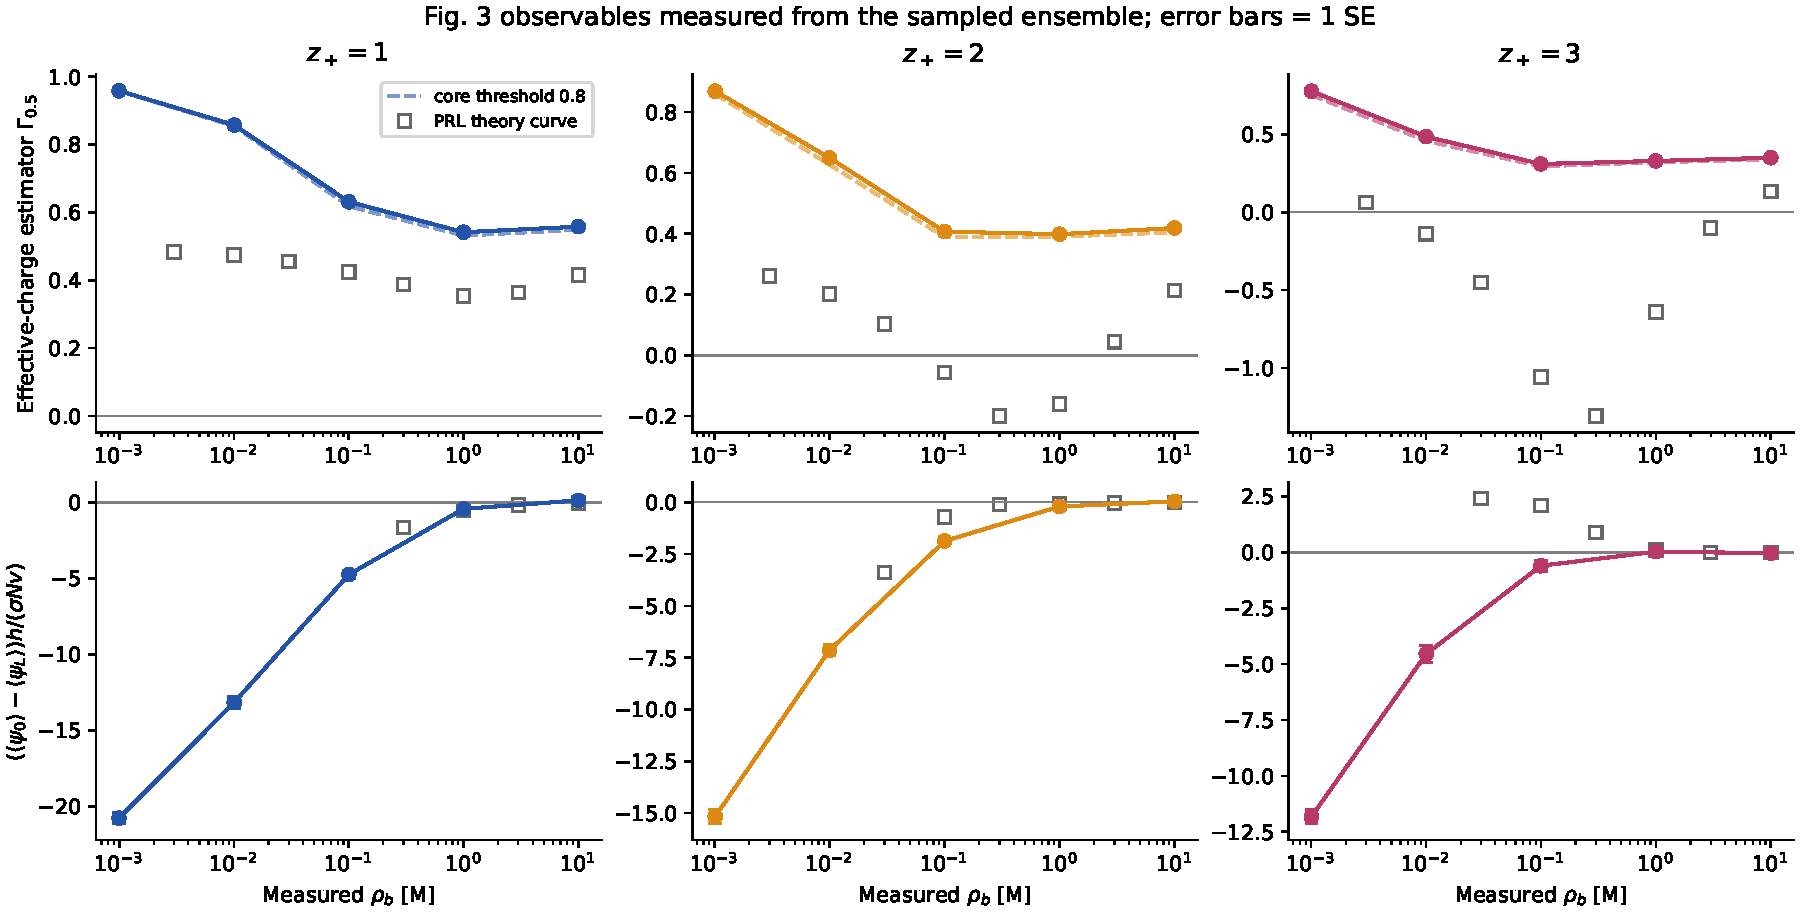
\includegraphics[width=\linewidth]{prl_comparison_figs/positive_brush_20260907/sampling_fig3.pdf}
\end{center}
\vspace{-7pt}
\smallnote{Solid: MC means with core threshold 0.5. Dotted: threshold 0.8. Open squares: PRL theory curves.
Surface potential uses the mean difference between first/last cell centers, without rescaling to fit the paper.}
\begin{align*}
 \overline\Gamma_c&=1-z_+
 \frac{\int_{\langle\rho_P\rangle>c\max\langle\rho_P\rangle}
       [\langle\rho_+\rangle-\rho_b]\,dz}
      {\int_{\langle\rho_P\rangle>c\max\langle\rho_P\rangle}
       \langle\rho_P\rangle\,dz},\\
 \Psi_{\rm rel}&=[\langle\psi(0)\rangle-\langle\psi(L)\rangle]
                  \frac{h}{\sigma Nv}.
\end{align*}
Observables are computed from mean profiles, rather than averaging nonlinear snapshot ratios.
Error estimates include recomputed core boundaries, shared bath uncertainty, and potential--height covariance.
$\Gamma$ differs from the actual net charge including C and anions, which is stored separately in the raw data.

\subhead{Finite-grid and cross-sectional-area controls}
Except for the salt-free row, $z_+=3$ and the target is $\rho_b=0.01\units{M}$.
Chain counts were adjusted with area to retain $\sigma=0.1\units{nm^{-2}}$.
Bulk activities were determined independently for each case.

\begin{tabularx}{\linewidth}{@{}Xrrr@{}}
\toprule
\rowcolor{panel}Control & $M$ & $A$ [nm$^2$] & $h$ [nm] \\
\midrule
\SamplingCheckRows
\bottomrule
\end{tabularx}

For all three valences, $\overline\Gamma_{0.5}$ was positive; potentials at $10\units{M}$ were within 2 SE of zero.
\textbf{Limits:} $A$ sets fluctuation strength in this 1D model, so varying area is more than
a numerical precision check. A few grid controls do not establish continuum convergence.
This restricted model has not reproduced the paper's contraction, re-expansion, and charge/potential reversal
from 3D charge correlations. These results also do not validate convergence of the original CL-FTS dynamics.
\smallnote{Code: \texttt{positive\_brush\_1d.py}, \texttt{run\_positive\_brush.py}.
Numbers, samples, and jobs: \texttt{dh\_salt\_runs/positive\_brush\_20260907/}.
Production FFT/C++/CUDA and the existing CL drift were unchanged in this work.
The following pages retain the earlier small-system and SCFT validation records.}

\clearpage
\pagetitle{Earlier checks: small systems and SCFT}{verdict}
\smallnote{Validation update: 2026-09-07\quad /\quad \texttt{devel/charged\_polymers}}

\begingroup\setlength{\fboxsep}{9pt}
\colorbox{panel}{\parbox{\dimexpr\linewidth-2\fboxsep\relax}{%
\textbf{Earlier validation verdict}\par
The real-field/particle sampler for a small finite 1D system is consistent with reference values.
PRL Figs.~1--3 were recalculated, but quantitative discrepancies remain.}}
\endgroup

\subhead{Models and scope of validation}
The 1D sampling in this section checks the existing finite 9-bead action. The PRL calculations use a separate
SCFT with $N=100$ chains, point ions, and incompressible P/S. These results do not validate the accuracy
of the existing complex Langevin (CL) dynamics or establish full PRL reproduction.

After exactly integrating the repulsive auxiliary field and electrostatic field $\psi$, a Gibbs sampler
retains particle positions and the real field in the attractive channel. Fields and positions are drawn
from their conditional distributions; integrating the field recovers the original particle action.
The next page gives this relation and the conditional mean and covariance.

\subhead{Controls for the same four-cell model}
Polymer density $\phi_{\mathrm P}$ in cell~1 for $M=4$, $E=25$.
Values following $\pm$ are standard errors (SE), accounting for blocking and autocorrelation.

\begin{tabularx}{\linewidth}{@{}Xr@{}}
\toprule
\rowcolor{panel}\textbf{Calculation} & \textbf{Mean $\pm$ SE} \\
\midrule
\DensityRows
\bottomrule
\end{tabularx}

\smallnote{The exact result sums $4^8=65{,}536$ particle configurations of the same action.
Historical CL values are stored results at $\Delta t=0.01$; the four-cell CL
$\Delta t\to0$ limit was not newly investigated here.}

\subhead{Completed calculations and the historical report}
There are 21 completed 1D sampling runs and 25 converged PRL Fig.~1 results. The Fig.~2--3
salt scans and unit/grid checks are appended below. Records of three initial failed Fig.~1
iterations are preserved; subsequent Newton/continuation runs converged for the same target equations.

\textbf{The original report appended to the combined PDF is historical.} Its claims of ``complete quantitative
reproduction,'' ``exact'' CL, and discrepancies due solely to LDA are superseded by the current validation
status. Production FFT and CL drift were unchanged during these checks.

\newpage
\pagetitle{Real-field integration and sampling}{equations}
Let $\bm R$ denote particle configurations and $\bm x$ a real field on $M$ cells.
$\bm\ell(\bm R)$ is the attractive-channel combination of smeared densities with its uniform mode removed.
Define the spatial mean and uniform-mode projection by
\begin{equation}
 \gridmean{f}=\frac{1}{M}\sum_{i=1}^{M}f_i,
 \qquad \gridmean{x}=\gridmean{\ell}=0,
 \qquad \Pi=I_M-\frac{\bm 1\bm 1^{\mathsf T}}{M}.
\end{equation}
Here $\bm 1$ is the all-ones vector and $\Pi$ projects onto the zero-mean subspace.
$a>0$ is the Gaussian coefficient of the attractive auxiliary field; $C>0$ is the action prefactor.
The $a$ on this page is distinct from the PRL Born radius.

\subhead{A joint distribution preserving the original particle weight}
Writing the original particle energy as $U_{\mathrm{particle}}(\bm R)$
and the chain bond weight as $B(\bm R)$ gives
\begin{align}
 U_{\mathrm{rep}}(\bm R)
 &= U_{\mathrm{particle}}(\bm R)
    +\frac{C}{4a}\,\gridmean{\ell(\bm R)^2}, \\
 P(\bm R,\bm x)
 &\propto B(\bm R)\,
    \exp\!\left[-U_{\mathrm{rep}}(\bm R)
    -C\,\gridmean{a x^2+\ell(\bm R)x}\right].
\end{align}
Completing the square,
\begin{equation}
 a x_i^2+\ell_i x_i
 =a\left(x_i+\frac{\ell_i}{2a}\right)^2-\frac{\ell_i^2}{4a}.
\end{equation}
integrating over $\mathcal X=\{\bm x:\bm 1^{\mathsf T}\bm x=0\}$ therefore gives,
up to a normalization independent of $\bm R$,
\begin{equation}
 \int_{\mathcal X}P(\bm R,\bm x)\,\mathrm d\bm x
 \propto B(\bm R)\exp[-U_{\mathrm{particle}}(\bm R)].
\end{equation}
The added quadratic term cancels exactly. This identity represents the same finite action;
it does not guarantee exact averages from a finite Monte Carlo trajectory.

\subhead{Field and particle updates}
For a fixed particle configuration, the Gaussian conditional distribution has
\begin{equation}
 \mathbb E[\bm x\mid\bm R]=-\frac{\bm\ell(\bm R)}{2a},
 \qquad
 \operatorname{Cov}(\bm x\mid\bm R)=\frac{M}{2Ca}\,\Pi.
\end{equation}
In practice, draw $\bm\eta\sim\mathcal N(\bm0,I_M)$ and set
$\bm x=-\bm\ell/(2a)+\sqrt{M/(2Ca)}\,\Pi\bm\eta$.
At fixed field, the conditional probability for a free particle at candidate position $r$ is
\begin{equation}
 P(R_j=r\mid\bm R_{-j},\bm x)
 =\frac{B(\bm R^{j\to r})\exp[-H(\bm R^{j\to r},\bm x)]}
 {\displaystyle\sum_{s=1}^{M}B(\bm R^{j\to s})\exp[-H(\bm R^{j\to s},\bm x)]},
 \qquad H=U_{\mathrm{rep}}+C\gridmean{a x^2+\ell x}.
\end{equation}
\smallnote{Each update sums only $M$ candidate positions, including all interactions and self terms,
neighboring bead bond weights, and the fixed first bead. Sampling requires no enumeration of all
$M^8$ configurations. The particle-only Gibbs control also integrates out the attractive field.}

\newpage
\pagetitle{Larger 1D grids and reference checks}{oned}
Parameters: $N_{\mathrm{ref}}=4$, 9 beads in total, $L=1$, $\chi N=2$, $\zeta N=4$,
and smearing radius $0.1$. The first bead is fixed in the first cell; bonds are reflecting.
Each run uses $2\times10^6$ sweeps, discards the first $2\times10^5$,
and stores every 10 sweeps, yielding $1.8\times10^5$ samples.

\begin{center}
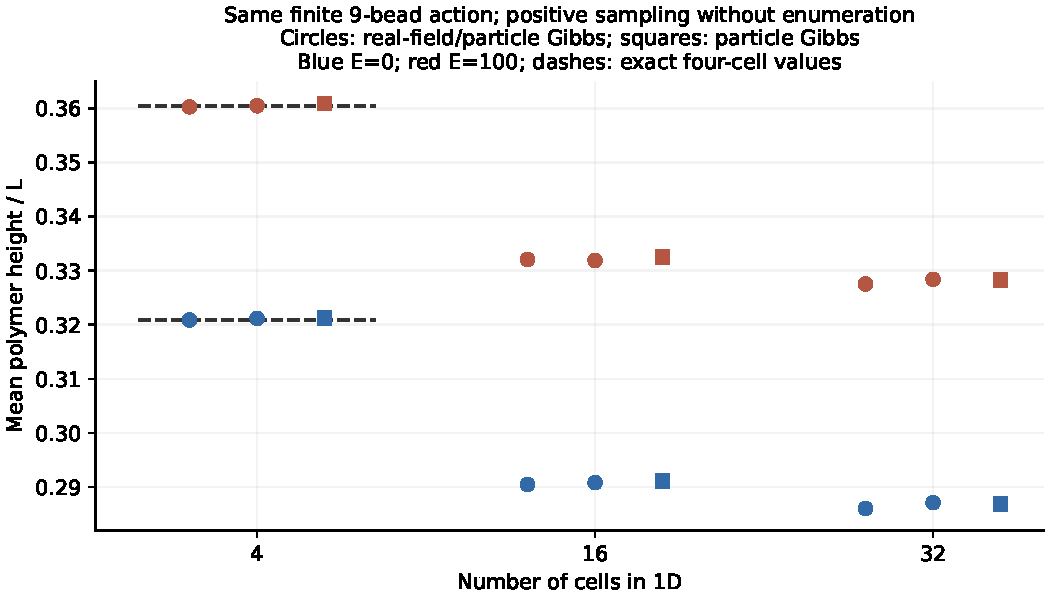
\includegraphics[width=.96\linewidth]{positive_1d_comparison.pdf}
\end{center}

\subhead{Mean height $\langle z\rangle/L$ at $E=100$}
{\small\setlength{\tabcolsep}{4pt}
\begin{tabularx}{\linewidth}{@{}l*{3}{>{\raggedleft\arraybackslash}X}@{}}
\toprule
\rowcolor{panel}Cells & Field/particle 1101 & Field/particle 1201 & Particle-only 2101 \\
\midrule
\HeightRows
\bottomrule
\end{tabularx}}

The exact four-cell height is $0.36049837$. In all nine $M=4$ runs, every measured quantity was
within $2.781\,\mathrm{SE}$ of its exact value. The largest difference between the two samplers across all runs
was $3.049$ combined SE. These are descriptive statistics over many correlated positions and observables,
not a claim that every individual $2\,\mathrm{SE}$ check passed.

\textbf{No exhaustive reference is available at $M=16,32$.} The two positive-probability samplers were compared.
The $16\to32$-cell height change exceeds statistical errors, so continuum convergence remains unverified.
The spatial representation of the first-cell anchor also changes with the grid.

\smallnote{Independent checks: Gaussian-integration energy identity error
$\le1.25\times10^{-14}$; conditional probability error for fields with standard deviation 5
$\le7.78\times10^{-16}$; species mass conserved in every sample. Local conditional field moments and
the sampled first cosine mode's mean and square were also checked. These small 9-bead results
do not validate performance for an actual $N=100$ brush.}

\newpage
\pagetitle{PRL Fig. 1: recalculated curves}{prl}
Paper parameters: $N=100$, $b=1\units{nm}$, $v=1\units{nm^3}$,
$\sigma=0.1\units{nm^{-2}}$, $a=0.25\units{nm}$,
$\ell_{\mathrm B}=0.7\units{nm}$, $\chi=0.5$, and $I_{\mathrm b}=0.3\units{M}$.
Primary runs use canonical monovalent counterions, GC salt, and $L=200\units{nm}$.
The graft is Gaussian with width $0.5b$; bonds use a truncated bottom and reflecting top.

\begin{center}
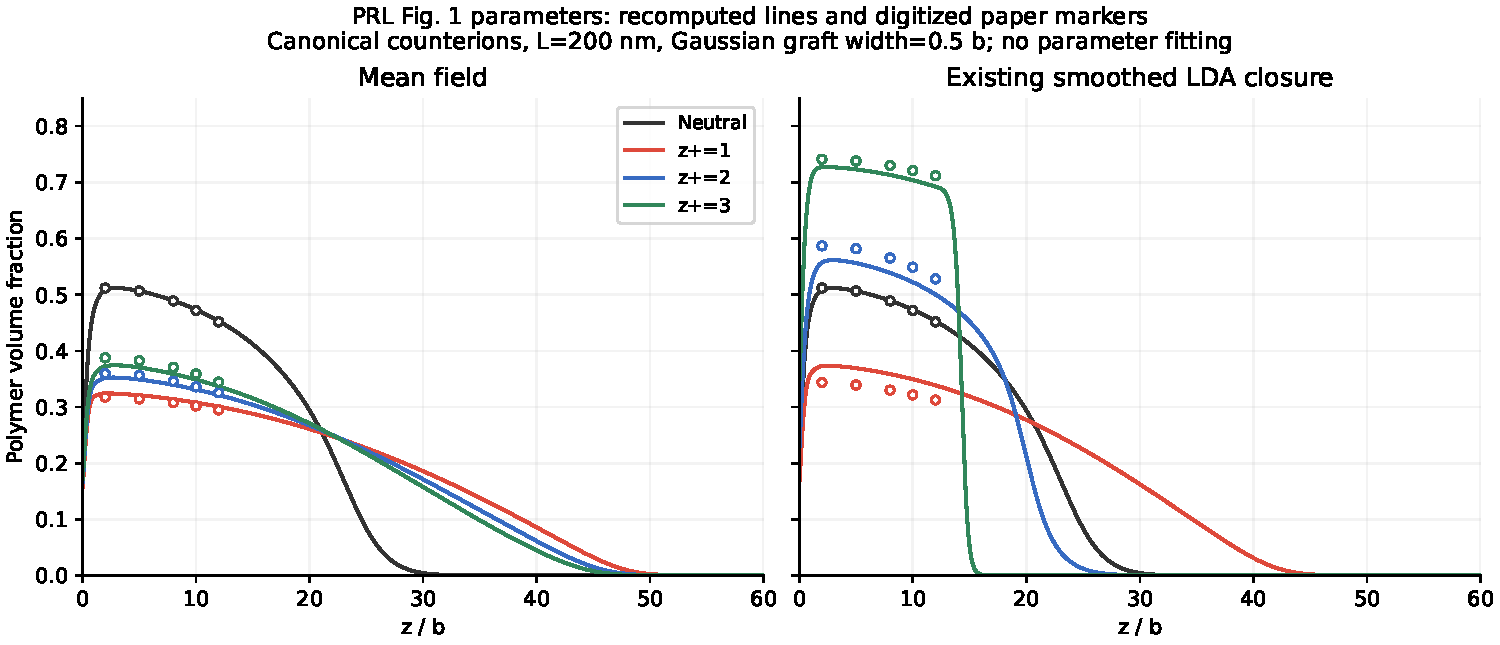
\includegraphics[width=\linewidth]{prl_fig1_checked.pdf}
\end{center}

\subhead{Polymer volume fraction $\phi_{\mathrm P}$ at $z/b=5$}
{\small
\begin{tabularx}{\linewidth}{@{}Xrr@{}}
\toprule
\rowcolor{panel}Curve & Paper (approx.) & This calculation, $N_z=3200$ \\
\midrule
\PrlRows
\bottomrule
\end{tabularx}}

Markers were read from the original PDF raster at $z/b=2,5,8,10,12$.
Estimated digitization uncertainty is about $\pm0.004$ in $\phi$, \textbf{not a statistical error}.
These are neither the authors' raw data nor an error assessment of the entire curves.

The maximum differences at the five interior positions for the three LDA curves are
$0.0300$, $0.0298$, and $0.0192$. At those positions, changes from $N_z=1600\to3200$
are at most $1.98\times10^{-5}$ in every case. The neutral curve and multivalent collapse trend agree,
but the observed grid error does not explain the discrepancies in the correlated curves.

\smallnote{Equal Born radii give $u_K=z_K^2U$, enabling coupled Newton equations for
$V=W/N$ and $U$. Convergence requires every residual of
$W$, Poisson, self-energy, and volume constraints to be below $10^{-7}$.
Independent chain density difference $\le5.67\times10^{-15}$;
contour partition error $\le4.96\times10^{-14}$.
The numerical graft/wall representation is not assumed identical to the paper's $\delta$ graft.}

\begin{landscape}
\thispagestyle{empty}
\pagetitle{Effects of correlation closure and ensemble}{closure}
\smallnote{Controls use the same Fig.~1 parameters. Neither LDA nor the current nonlocal backend
has been validated as an implementation of the full SI theory.}
\begin{center}
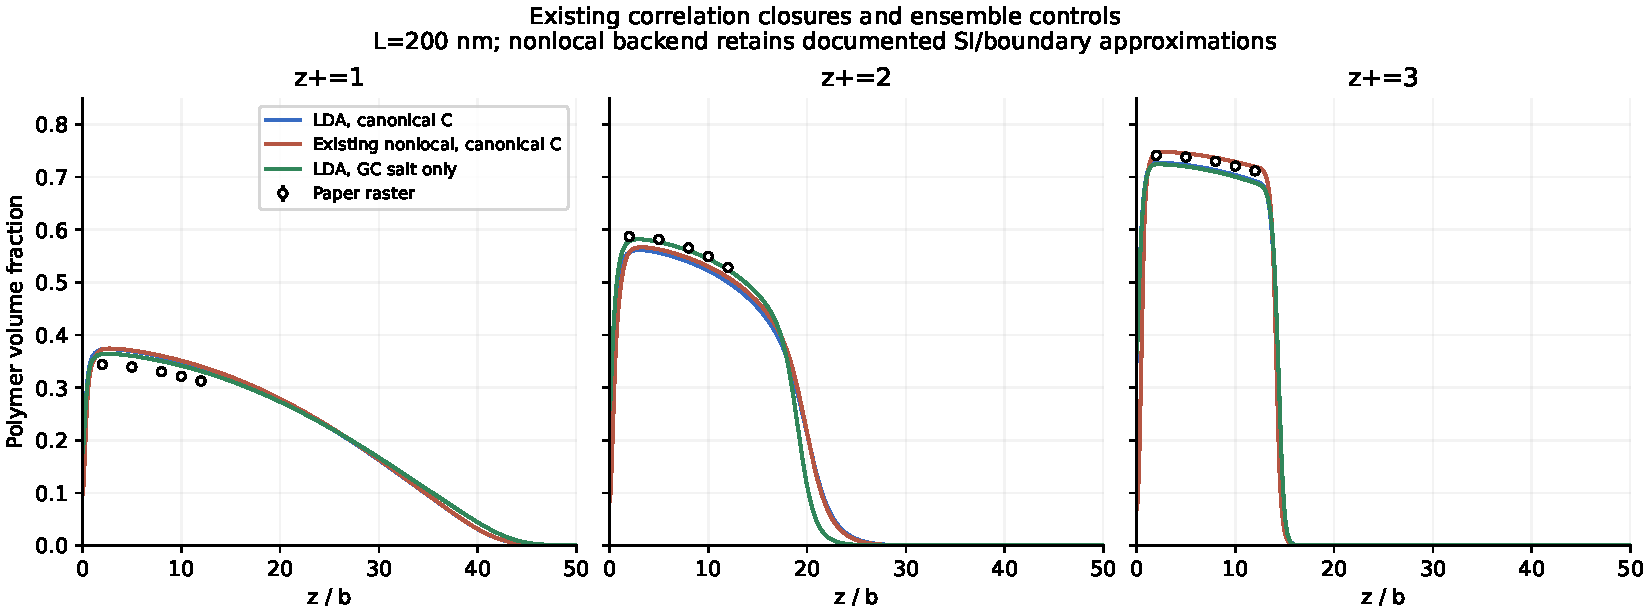
\includegraphics[width=.94\linewidth]{prl_closure_comparison.pdf}
\end{center}
\vspace{-6pt}
\begin{minipage}[t]{.48\linewidth}
\raggedright
\textbf{Maximum $|\Delta\phi|$ from the paper: five interior positions}

{\small\setlength{\tabcolsep}{4pt}
\begin{tabularx}{\linewidth}{@{}l*{3}{>{\raggedleft\arraybackslash}X}@{}}
\toprule
\rowcolor{panel}$z_+$ & LDA + C & LDA GC-only & nonlocal + C \\
\midrule
\ClosureRows
\bottomrule
\end{tabularx}}

\smallnote{C denotes canonical monovalent counterions. GC-only mean field agrees to within
$0.0027$ at the same positions.
For $L=200\to400\units{nm}$, the LDA height $2\langle z\rangle$ changes by
$30.9787\to31.3638\units{nm}$ at $z_+=1$ and
$14.3395\to14.3667\units{nm}$ at $z_+=3$.
This moment height is not the Gibbs height of Fig.~2.}
\end{minipage}\hfill
\begin{minipage}[t]{.48\linewidth}
\raggedright
\textbf{Remaining discrepancies and reproduction scope}

\small
Trivalent nonlocal SCFT converged after continuation, with residuals below $4.61\times10^{-9}$.
Omitted $I_{\mathrm{ex}}$, Green-function boundary and smearing approximations,
and quadrature/grid validation remain unresolved. Quantitative reproduction for all three valences is incomplete.

\smallnote{This page checks Fig.~1. New Fig.~2--3 calculations follow;
Fig.~4 was not recalculated in this work.
Details: \texttt{ONED\_PRL\_REPRODUCTION.md}. Raw data are in
\texttt{\textasciitilde/polymer/dh\_salt\_runs/oned\_prl\_20260907/}:
\texttt{comparison.json}, \texttt{prl\_comparison.csv}, run scripts, and SLURM logs.
Paper: \href{https://doi.org/10.1103/PhysRevLett.134.048101}{Duan et al., PRL 134, 048101 (2025)}.}
\end{minipage}
\vfill
{\scriptsize\color{muted}\hrule\vspace{5pt}
Validation update \enspace|\enspace 2026-09-07\hfill\thepage\par}
\end{landscape}

% Editable continuation of ONED_PRL_REPRODUCTION.tex.
% Numerical macros and vector figures are refreshed by the PDF builder.
% Generated from the Fig. 2-3 comparison.json.
\newcommand{\FigTwentyThreePrimaryCount}{57}
\newcommand{\FigTwentyThreePairedCount}{57}
\newcommand{\FigTwentyThreeExtendedCheckedCount}{215}
\newcommand{\FigTwentyThreeFailedCount}{47}
\newcommand{\FigTwentyThreeSaltfreeMoment}{$50.91$}
\newcommand{\FigTwentyThreeSaltfreeEquimolar}{$38.45$}
\newcommand{\FigTwentyThreeNeutralMoment}{$21.78$}
\newcommand{\FigTwentyThreeFullResidual}{$6.02\times10^{-8}$}
\newcommand{\FigTwentyThreeChainError}{$2.33\times10^{-13}$}
\newcommand{\FigTwentyThreeContourError}{$1.98\times10^{-12}$}
\newcommand{\FigTwentyThreeMassError}{$3.55\times10^{-15}$}
\newcommand{\FigTwentyThreeCounterionMassError}{$3.55\times10^{-15}$}
\newcommand{\FigTwentyThreePairHeightDifferenceNm}{$2.85\times10^{-7}$}
\newcommand{\FigTwentyThreePairGammaDifference}{$2.90\times10^{-9}$}
\newcommand{\FigTwentyThreePairPsiDifference}{$6.81\times10^{-9}$}
\newcommand{\FigTwentyThreePairDensityDifference}{$1.90\times10^{-8}$}
\newcommand{\FigTwentyThreePairPotentialProfileDifference}{$2.71\times10^{-8}$}
\newcommand{\FigTwentyThreeMinimaRows}{%
$1$ & $50$ & $21.91$ & $-0.3661$ \\
$2$ & $0.1$ & $19.51$ & $-0.4165$ \\
$3$ & $0.03162$ & $14.11$ & $-0.5572$ \\
}
\newcommand{\FigTwentyThreeGridRows}{%
$1$ & $0$ & $8.02\times10^{-4}$ & $0.01049$ \\
$1$ & $1.00\times10^{-7}$ & $8.02\times10^{-4}$ & $0.009946$ \\
$2$ & $0.1$ & $0.00221$ & $-0.5041$ \\
$3$ & $0.01$ & $0.003446$ & $-0.3023$ \\
$3$ & $10$ & $0.001948$ & $-5.11\times10^{-5}$ \\
}

\clearpage
\pagetitle{Fig. 2: contraction and re-expansion}{figtwo}
\smallnote{Additional calculations: 1D smoothed-LDA SCFT at fixed parameters. These do not validate
the paper's full SI theory or the existing CL dynamics.}

For each $z_+=1,2,3$, 19 standard points span $10^{-7}\le\rho_b\le50\units{M}$;
validated solutions were obtained at \FigTwentyThreePrimaryCount/57 points.
Upward/downward concentration continuation and intermediate points used separate SLURM jobs.
No valence-dependent background salt concentration or height correction was fitted.

\begin{center}
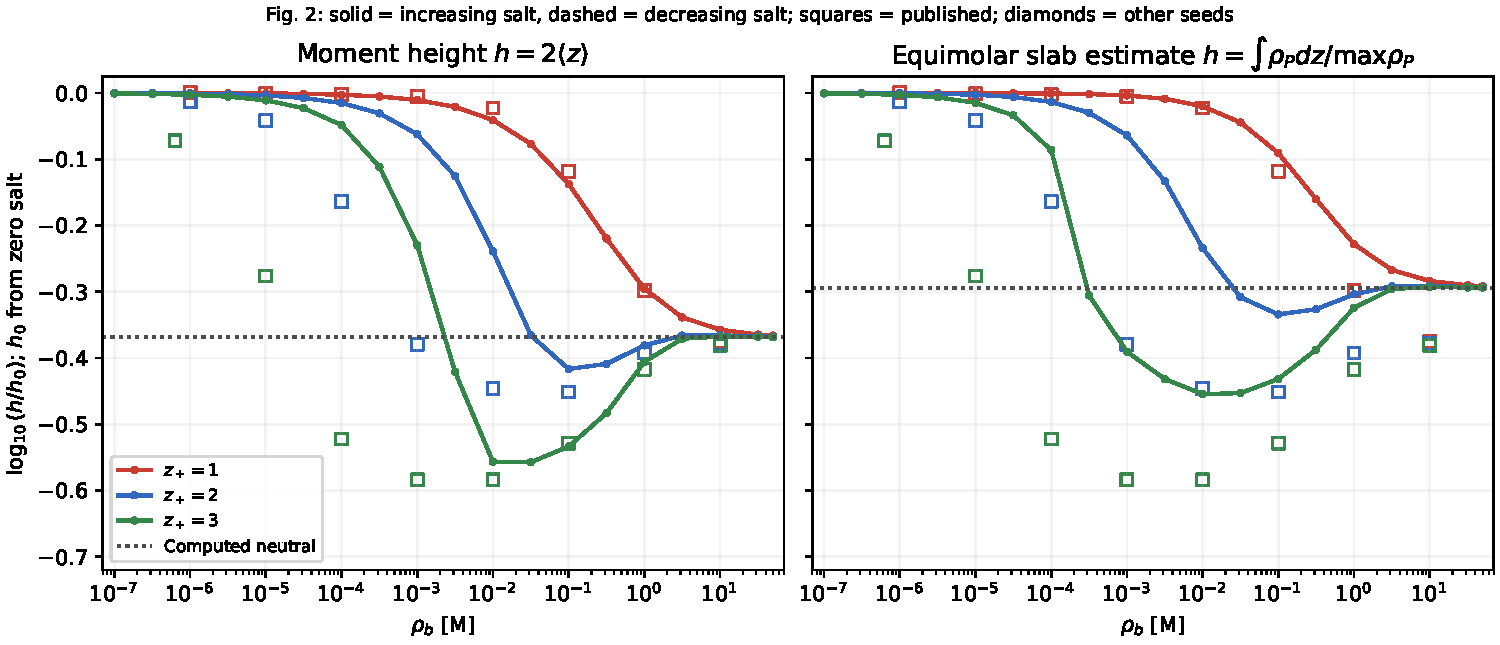
\includegraphics[width=\linewidth]{prl_comparison_figs/fig23_prl_20260907/fig2_checked.pdf}
\end{center}
\vspace{-7pt}
\smallnote{Solid/dotted: upward/downward scans. Open squares: digitized paper theory curves.
Diamonds mark points obtained only from separate initial states, if any. Experimental symbols were excluded.
Digitization uncertainty is about $0.01$ in $\log_{10}(h/h_0)$, not a statistical error.}

\subhead{Explicit height definitions and salt-free references}
\begin{equation*}
 h_{\rm m}=\frac{2\int z\rho_{\rm P}(z)\,dz}{\sigma N},\qquad
 h_{\rm eq}=\frac{\sigma N}{\max_z\rho_{\rm P}(z)},\qquad
 \int\rho_{\rm P}(z)\,dz=\sigma N=10\units{nm^{-2}}.
\end{equation*}
$h_{0,\rm m}=$\FigTwentyThreeSaltfreeMoment\,nm,
$h_{0,\rm eq}=$\FigTwentyThreeSaltfreeEquimolar\,nm were obtained by
solving $\rho_b=0$ directly. The neutral brush has moment height
\FigTwentyThreeNeutralMoment\,nm.
The paper mentions a Gibbs dividing surface without specifying the extraction procedure or reference density.
Neither definition above is therefore assumed equal to the paper's Gibbs height.

\subhead{Minimum moment heights among the 19 standard points}
\begin{tabularx}{\linewidth}{@{}Xrrr@{}}
\toprule
\rowcolor{panel}$z_+$ & $\rho_b$ [M] & $h_{\rm m}$ [nm] & $\log_{10}(h_{\rm m}/h_{0,\rm m})$ \\
\midrule
\FigTwentyThreeMinimaRows
\bottomrule
\end{tabularx}
\smallnote{These are sampled minima, not exact minima over continuous concentration. The monovalent minimum is at the scan limit.
Multivalent contraction and re-expansion occur, but the onset of contraction at low salt differs from the paper.
Changing the height definition does not produce simultaneous quantitative agreement for all three curves.}

\clearpage
\pagetitle{Fig. 3: effective charge and potential}{figthree}
\smallnote{SCFT profile observables are distinguished from direct evaluation of the paper's Eqs.~(7) and (9).}
\begin{center}
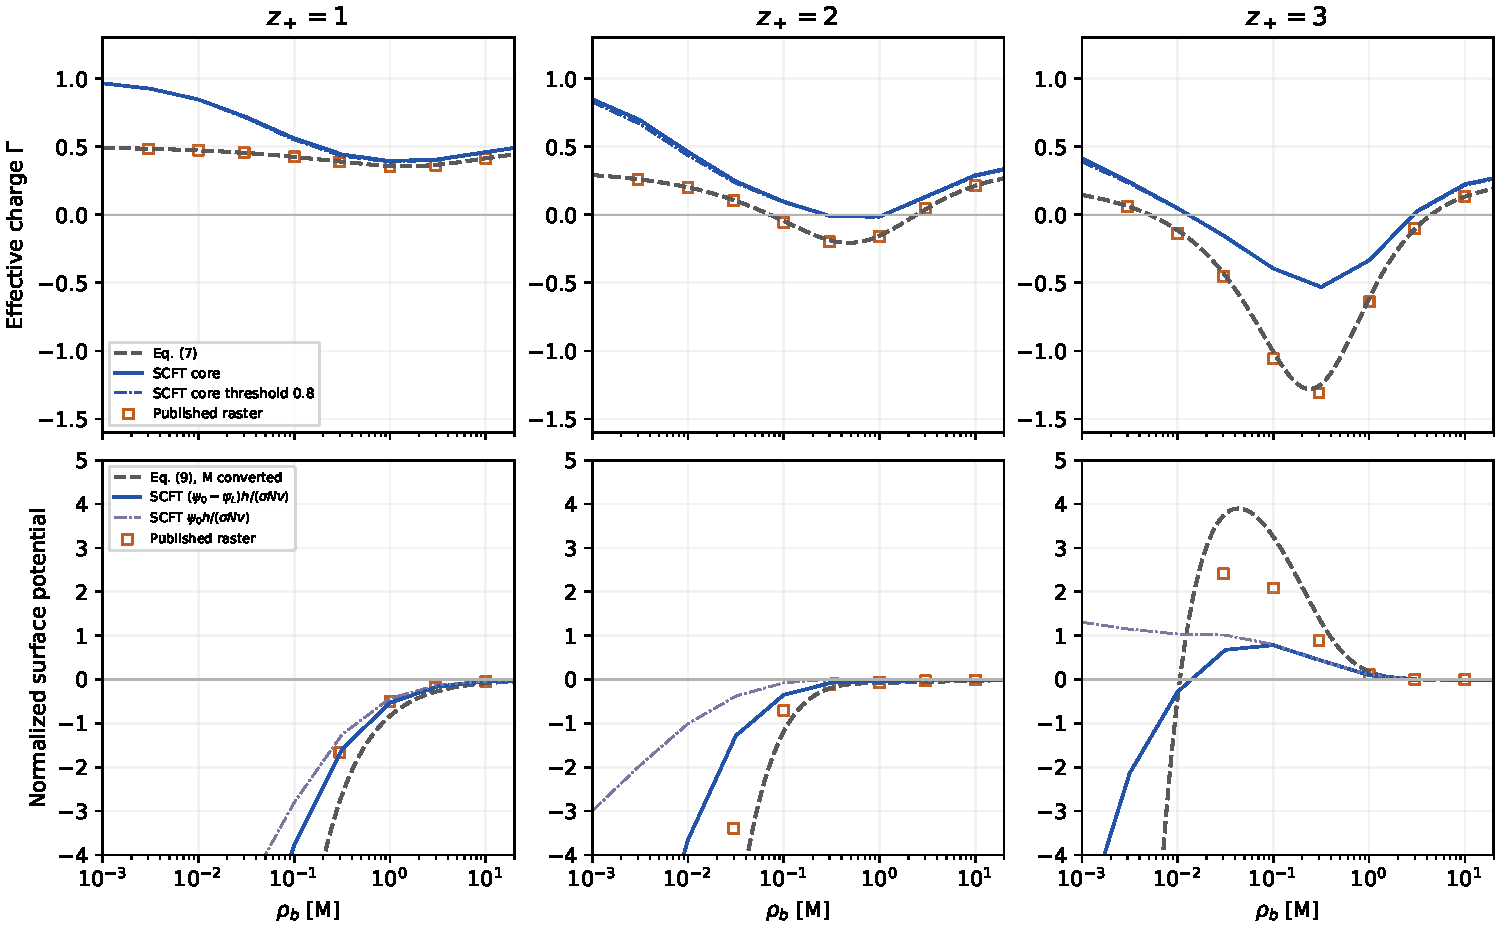
\includegraphics[width=\linewidth]{prl_comparison_figs/fig23_prl_20260907/fig3_checked.pdf}
\end{center}
\vspace{-5pt}
\smallnote{Gray dashed: analytical formulas. Squares: paper curves. Blue: SCFT.
Solid/dotted SCFT lines show upward/downward scans. Large negative potentials outside the plotting range are clipped.}

\subhead{Observables measured from SCFT}
\begin{align*}
 \Gamma(z)&=1-z_+\frac{\rho_+(z)-\rho_b}{\rho_{\rm P}(z)},
 &\overline\Gamma_c&=
 \frac{\int_{\rho_{\rm P}>c\rho_{\rm P}^{\max}}\rho_{\rm P}(z)\Gamma(z)\,dz}
 {\int_{\rho_{\rm P}>c\rho_{\rm P}^{\max}}\rho_{\rm P}(z)\,dz},\\
 \Psi_{\rm rel}&=[\psi(0)-\psi(L)]\frac{h_{\rm m}}{\sigma Nv},
 &\Psi_0&=\psi(0)\frac{h_{\rm m}}{\sigma Nv}.
\end{align*}
Both core thresholds, $c=0.5$ and $0.8$, are plotted. These explicit averages of nonuniform profiles
are not automatically equivalent to the paper's uniform-brush scaling variables.

The finite box contains a fixed number of monovalent counterions, allowing $\psi(L)\ne0$.
We therefore record both $\Psi_0$ relative to zero and the wall--far-end difference $\Psi_{\rm rel}$.
The sign of $\psi(0)$ alone does not establish charge inversion, particularly at low salt.
Wall/far-end potentials are approximated by first/last cell-center values.

\subhead{Analytical formulas and SCFT have different scopes}
SI Eq.~(S34) assumes high salt, $\rho_b\gg\rho_{\rm P}$, with negligible canonical counterion effects.
Low-salt SCFT does not satisfy these conditions.
Reproducing the analytical formulas therefore does not validate SCFT or CL.
The current LDA must be compared with the paper's nonlocal Green function/$I^{\rm ex}$ treatment.
The paper also neglects $u_{\rm P}^{\rm ex}$ for brushes; that omission alone is not an established cause of the discrepancy.

\smallnote{Among the 19 standard points, the divalent core $\Gamma$ reaches $-0.0140$, while $\Psi_{\rm rel}$
remains negative. For trivalent salt, $\Gamma_{\min}\simeq-0.5314$ and $\Psi_{{\rm rel},\max}\simeq+0.7834$.
Overcharging and potential reversal are qualitatively distinct, but the trivalent potential peak differs from the paper's value of about 2.5.}

\clearpage
\pagetitle{Checking Fig. 3 potential normalization}{figthreeunits}
\smallnote{A diagnostic of the equation--figure discrepancy. The scale factor below was not applied to SCFT results.}
The paper's Gaussian charge-spread function and Eqs.~(7), (9) were evaluated as follows.
\begin{align*}
 u(x)&=1-x\,\operatorname{erfcx}(x/\sqrt\pi),
 &u'(x)&=-\left(1+\frac{2x^2}{\pi}\right)\operatorname{erfcx}(x/\sqrt\pi)+\frac{2x}{\pi},\\
 \kappa_b^2&=4\pi\ell_B z_+(z_++1)\rho_b,
 &R&=-\frac{z_+(z_++1)\kappa_b\ell_B}{4}u'(a\kappa_b),\\
 \Gamma&=\frac{1-R}{z_++1-R},
 &\Psi_{\rm Eq.9}&=-\frac{(z_+^2-1)\Gamma+1}{z_+^2(z_++1)v\rho_b}.
\end{align*}
Parameters are $a=0.25\units{nm}$, $\ell_B=0.7\units{nm}$, and $v=1\units{nm^3}$.
The formulas use number density $\rho_b[\mathrm{nm^{-3}}]=0.6022\,\rho_b[\mathrm M]$.

\begin{center}
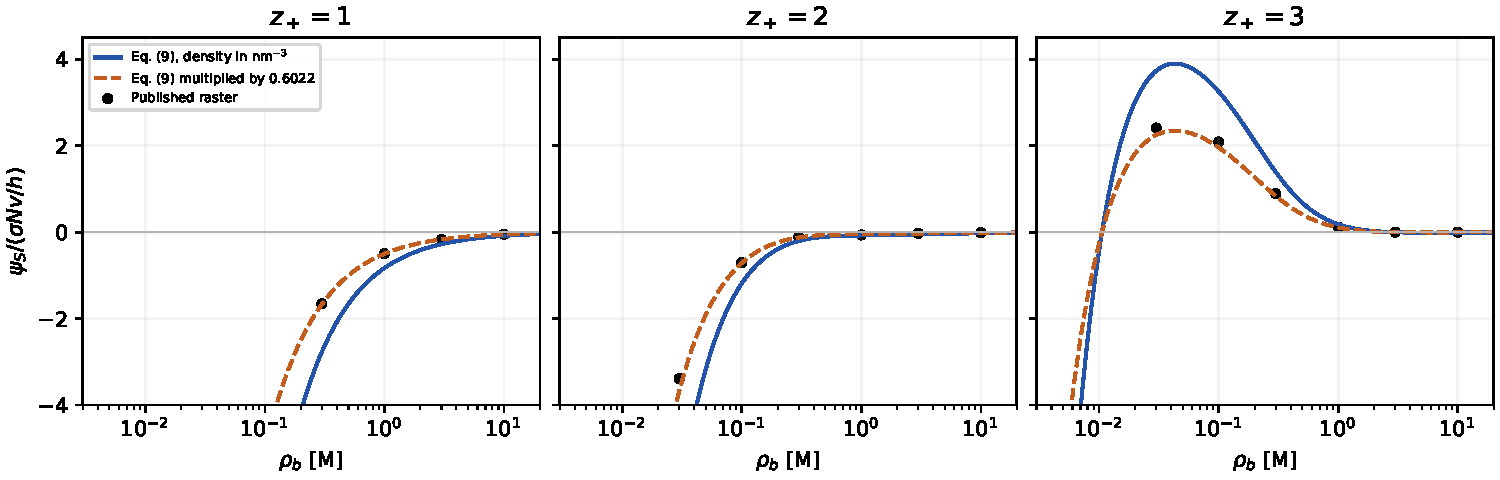
\includegraphics[width=\linewidth]{prl_comparison_figs/fig23_prl_20260907/fig3_units_check.pdf}
\end{center}
\vspace{-6pt}
\smallnote{Blue: Eq.~(9) with unit conversion. Orange dotted: that value multiplied by 0.6022, for diagnosis only.
Black dots: digitized original raster. The latter scale equals omitting the density conversion in the denominator;
it is not asserted to be the correct physical normalization.}

\subhead{The monovalent check is independent of correlation parameters}
For $z_+=1$, $\Psi_{\rm Eq.9}=-1/(2v\rho_b)$, eliminating $a,\ell_B,\Gamma$.

\begin{tabularx}{\linewidth}{@{}Xrrr@{}}
\toprule
\rowcolor{panel}$\rho_b$ [M] & Eq.~(9), converted & Paper (approx.) & Eq.~(9)$\times0.6022$ \\
\midrule
$0.3$ & $-2.7676$ & $-1.6598$ & $-1.6667$ \\
$1$ & $-0.8303$ & $-0.4985$ & $-0.5000$ \\
$3$ & $-0.2768$ & $-0.1701$ & $-0.1667$ \\
\bottomrule
\end{tabularx}

The monovalent discrepancy is consistent with the M--nm$^{-3}$ conversion factor. Multivalent discrepancies remain.
\textbf{The units/normalization connecting the paper's equations and figure require confirmation.}
The cause is not established without the authors' raw data or plotting code.
\smallnote{Source: \href{https://doi.org/10.1103/PhysRevLett.134.048101}{Duan et al., PRL 134, 048101 (2025)},
Eqs.~(7), (9), Fig.~3, and SI Eqs.~(S33), (S38). The printed SI Eq.~(S42) lacks the
$\rho_b$ denominator visible in main-text Eq.~(9); potentials were therefore evaluated from the main-text equation.}

\clearpage
\pagetitle{Numerical checks and remaining gaps}{figtwothreechecks}
\subhead{Numerical issues addressed in a separate Python research runner}
The existing real-space chain calculation also suffered floating-point underflow at low salt.
Densities differed from an independent log-space calculation by up to $0.2098\units{nm^{-3}}$,
hidden by per-bead floors and final mass normalization.
The new runner evaluates positive bond convolutions in extended precision,
using one partition function for every contour position.
Independent log-sum-exp calculations check final densities and contour consistency.

The runner adds Poisson--Boltzmann Newton updates including derivatives of canonical C normalization.
The Jacobian is tridiagonal plus a rank-one term.
For random fields (std $\simeq5$), its relative finite-difference error was $3.77\times10^{-10}$.
These changes are confined to \texttt{run\_prl\_fig23\_checked.py}.
Production FFT/C++/CUDA, CL drift, and the existing \texttt{prl\_scft.py} were unchanged in this work.

\subhead{Acceptance criteria and maximum observed errors}
\begin{tabularx}{\linewidth}{@{}Xrr@{}}
\toprule
\rowcolor{panel}Check & Required & Observed maximum \\
\midrule
Full SCFT residual & $10^{-7}$ & \FigTwentyThreeFullResidual \\
Independent chain density difference & $10^{-10}$ & \FigTwentyThreeChainError \\
Relative contour partition error & $10^{-10}$ & \FigTwentyThreeContourError \\
Polymer integral error [nm$^{-2}$] & $10^{-10}$ & \FigTwentyThreeMassError \\
Canonical C integral error [nm$^{-2}$] & $10^{-10}$ & \FigTwentyThreeCounterionMassError \\
\bottomrule
\end{tabularx}
\FigTwentyThreeExtendedCheckedCount{} extended-precision runs passed validation.
Failed attempts are excluded from successful results; their logs and checkpoints are preserved.
Across \FigTwentyThreePairedCount{} upward/downward pairs at matching concentrations,
the largest height difference is \FigTwentyThreePairHeightDifferenceNm\,nm.
The maximum full polymer density profile difference is \FigTwentyThreePairDensityDifference\,nm$^{-3}$.
This checks iterative solution consistency; it does not prove a free-energy minimum.

\subhead{Grid and box size: moment height changes [nm]}
The reference is $L=200\units{nm}$, $N_z=1600$. Grid refinement uses $N_z=3200$;
box enlargement uses $L=400\units{nm}$, $N_z=3200$.

\begin{tabularx}{\linewidth}{@{}Xrrr@{}}
\toprule
\rowcolor{panel}$z_+$ & $\rho_b$ [M] & $\Delta h$, finer grid & $\Delta h$, larger box \\
\midrule
\FigTwentyThreeGridRows
\bottomrule
\end{tabularx}
\smallnote{These are selected-point checks, not proof of $L\to\infty$ convergence for the full scan.
One failed high-salt PB residual check was rerun with a tighter inner PB tolerance.
The SCFT acceptance threshold was not relaxed.}

\smallnote{Raw data: \texttt{\textasciitilde/polymer/dh\_salt\_runs/fig23\_prl\_20260907/}.
Preserved files include \texttt{comparison.json}, \texttt{fig23\_primary.csv}, each job's \texttt{run.sh},
\texttt{summary.json}, \texttt{profiles.npz}, SLURM logs, and digitized figure coordinates.
Reproduction steps and limitations are recorded in \texttt{FIG23\_PRL\_REPRODUCTION.md}.}


% The combined report compiles this same source, then appends the archive.
% This preserves the landscape page at full size and keeps one editable body.
\ifdefined\IncludeHistoricalReport
\clearpage
\hypersetup{pdftitle={PRL comparison with current validation update}}
\newcommand{\HistoricalBanner}{%
  \AddToShipoutPictureFG*{\AtPageUpperLeft{%
    \put(24,-18){\makebox[0pt][l]{\fontsize{7.2}{9}\selectfont\color{red!65!black}%
      HISTORICAL REPORT --- superseded validation status; see the update at the start of this PDF.}}}}}
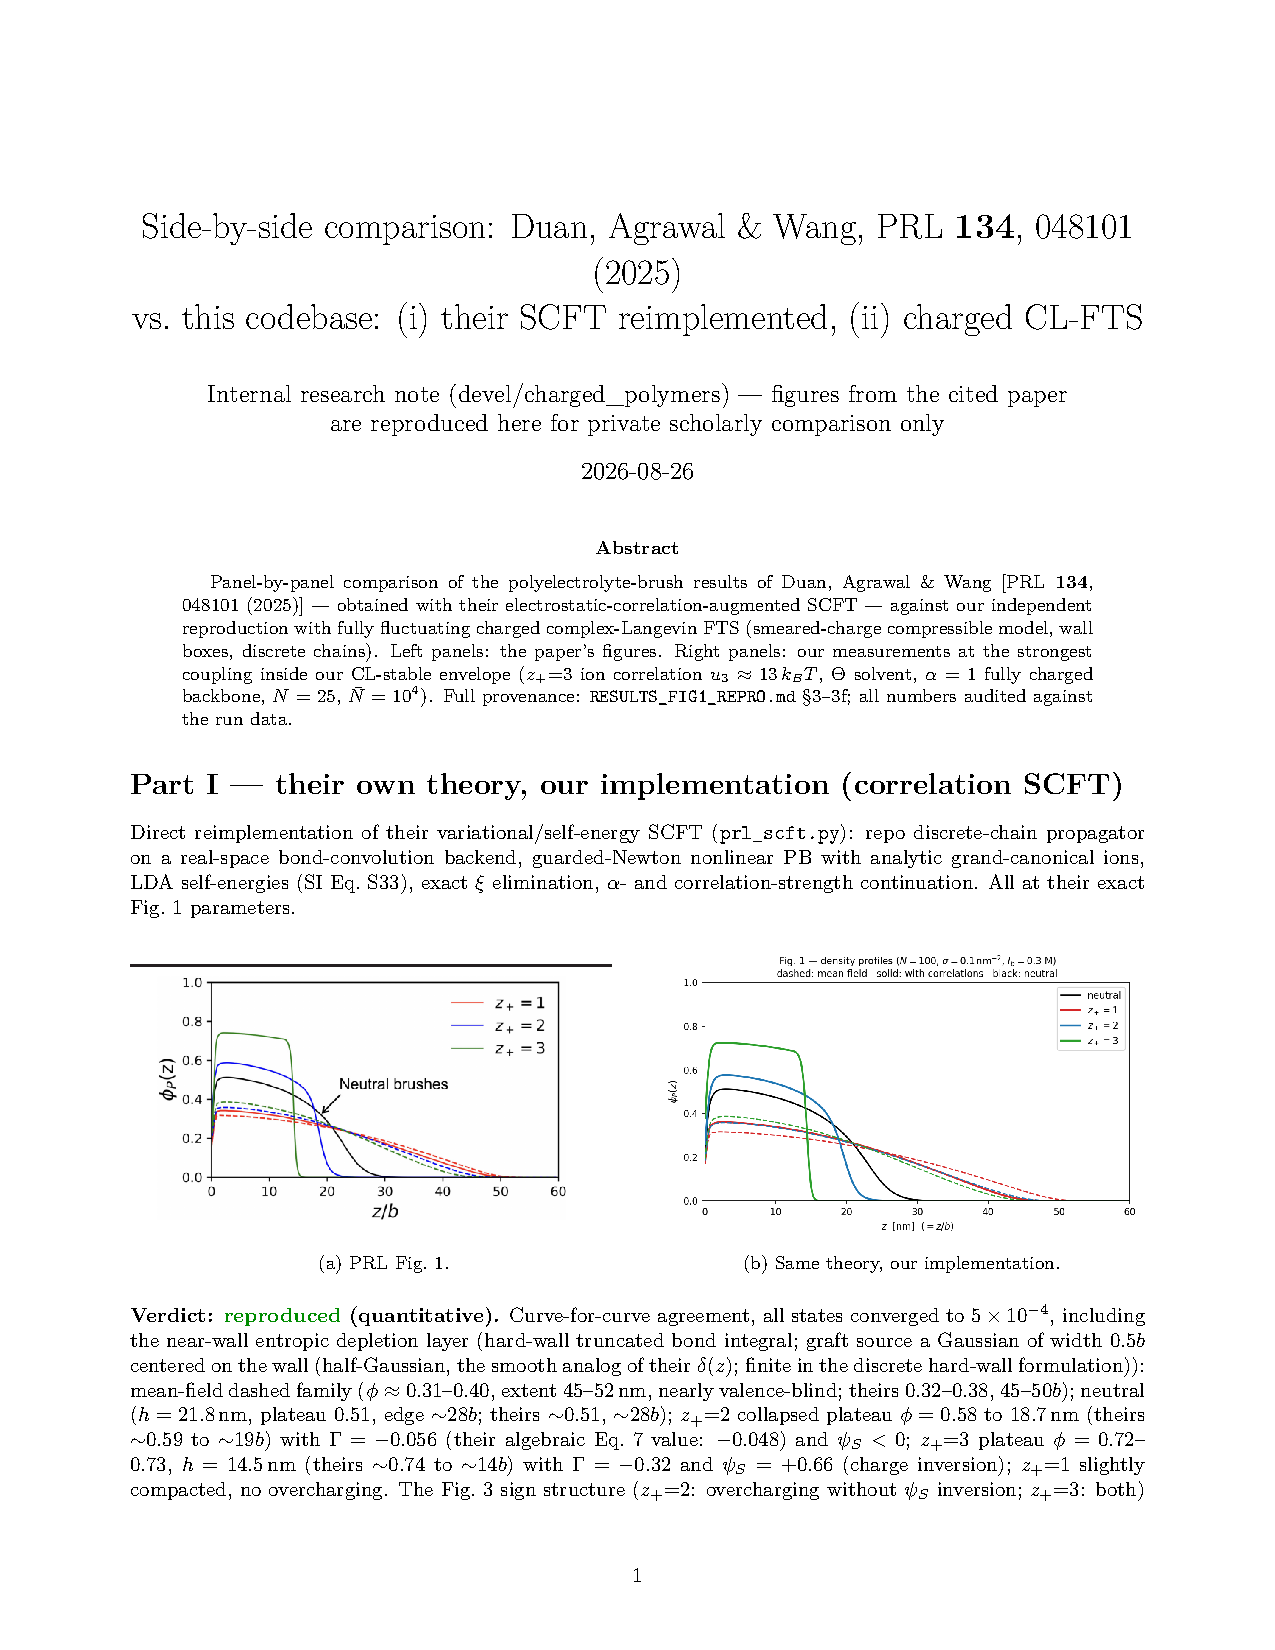
\includepdf[pages=-,fitpaper=true,pagecommand={\thispagestyle{empty}\HistoricalBanner},
  addtotoc={1,section,1,{Original comparison report: historical record},historical}]
  {prl_comparison_figs/archive/PRL_COMPARISON_before_20260907_update.pdf}
\fi
\end{document}
